%
% First comes an example EPS file -- just ignore it and
% proceed on the \documentclass line
% your LaTeX will extract the file if required
\begin{filecontents*}{example.eps}
%!PS-Adobe-3.0 EPSF-3.0
%%BoundingBox: 19 19 221 221
%%CreationDate: Mon Sep 29 1997
%%Creator: programmed by hand (JK)
%%EndComments
gsave
newpath
  20 20 moveto
  20 220 lineto
  220 220 lineto
  220 20 lineto
closepath
2 setlinewidth
gsave
  .4 setgray fill
grestore
stroke
grestore
\end{filecontents*}
%
\RequirePackage{fix-cm}
%
% \documentclass{svjour3}                     % onecolumn (standard format)
%\documentclass[smallcondensed]{svjour3}     % onecolumn (ditto)
\documentclass[smallextended]{svjour3}       % onecolumn (second format)
%\documentclass[twocolumn]{svjour3}          % twocolumn
%
\smartqed  % flush right qed marks, e.g. at end of proof
%
\usepackage{graphicx}
\usepackage[most]{tcolorbox}
\usepackage{listings}
\usepackage{xcolor}
\usepackage{subcaption}
\usepackage{tabularx}
\usepackage{booktabs}
\usepackage[colorinlistoftodos,prependcaption,textsize=tiny]{todonotes}
\usepackage{wrapfig}

\definecolor{backcolor}{rgb}{0.95,0.95,0.92}
\colorlet{punct}{red!60!black}
\definecolor{delim}{RGB}{20,105,176}
\colorlet{numb}{magenta!60!black}

\lstdefinestyle{mystyle}{
  language=Python,
  basicstyle=\ttfamily\footnotesize,
  keywordstyle=\color{delim},
  stringstyle=\color{punct},
  commentstyle=\color{numb},
  breakatwhitespace=true,
  breaklines=true,
  keepspaces=true,
  showspaces=false,
  showstringspaces=false,
  showtabs=false,
  tabsize=2,
  stepnumber=1,
  numbersep=3pt,
  captionpos=b,
  numbers=left,
  numberstyle=\tiny\color{gray},
  backgroundcolor=\color{backcolor},
  aboveskip=0pt,
  belowskip=0pt
}
\lstset{style=mystyle}

\lstset{emph={%  
    assert%
    },emphstyle={\color{delim}}%
}%

%
% \usepackage{mathptmx}      % use Times fonts if available on your TeX system
%
% insert here the call for the packages your document requires
%\usepackage{latexsym}
% etc.
%
% please place your own definitions here and don't use \def but
% \newcommand{}{}
%
% Insert the name of "your journal" with
% \journalname{myjournal}
%
\begin{document}

\title{Exploring the Role of Feedback in Machine Learning Jupyter Notebooks}

%\titlerunning{Short form of title}        % if too long for running head

\author{Arumoy Shome\and
  Lu{\`\i}s Cruz\and
  Diomidis Spinellis\and
  Arie van Deursen
}

%\authorrunning{Short form of author list} % if too long for running head

\institute{A. Shome \at
  Delft University of Technology\\
  \email{a.shome@tudelft.nl}
  \and
  L. Cruz \at
  Delft University of Technology\\
  \email{l.cruz@tudelft.nl}
  \and
  D. Spinellis \at
  Delft University of Technology\\
  \email{d.spinellis@tudelft.nl}
  \and
  A. V. Deursen \at
  Delft University of Technology\\
  \email{arie.vandeursen@tudelft.nl}
}

\date{Received: date / Accepted: date}
% The correct dates will be entered by the editor


\maketitle

\begin{abstract}

  \todo{update the numbers here}
Testing ML systems is a highly interactive process which demands a human-in-the-loop approach. In addition to writing tests for the code base, practitioners are required to analyse and interpret several visualisations using their domain expertise to validate if an ML system satisfies the required set of functional and non-functional properties. Visualisations are frequently used to qualitatively assess various parts of an ML pipeline. However, implicit knowledge gained from visualisations must be translated to explicit analytical tests that fail when there is change in any component of the ML pipeline. We conduct an empirical analysis of Jupyter notebooks to catalogue the state-of-the-art mappings between ML visualisations and assertions. We mine Github to collect 54K Jupyter Notebooks that contain assertions written in Python. We develop a novel methodology to identify 1764 notebooks which contain an assertion below a visualisation. We manually analyse the 1.7K notebooks and identify 269 visualisation-assertion pairs that are semantically related to one another. We further investigate the 269 visualisation-assertion pairs and identify three frequently occurring testing patterns. We perform an in-depth analysis of 34 visualisation-assertion pairs and find that the assertions often fail to capture all the information present in their visual counter-part. Empirical evidence obtained in this study indicates that current software testing methods fail to address the unique challenges of ML. And emphasises the need for automated tools that bridge the gap between visual assessments and analytical assertions.

\keywords{ML Testing \and SE4AI \and Visualisations \and Assertions \and Computational Notebooks}
\end{abstract}

\section{Introduction}

% amershi2019software: start with ML development life cycle and how everything is done in a very iterative way; things are dependant on one another; etc.

% martinez-plumed2021crisp-dm: not only does ML include the crip-dm framework, but this same form of iteration is seen in the model development and experimentation phase;

% this is why we see the use of computational notebooks being widely adopted by the ML community

% writing ML code is more iterative and requires a constant feedback; we identify this feedback can be provided in two ways: implicitly from the output of a cell and explicitly from a failed assertion

Code, data and ML model in ML-enalbed systems are highly tangled with each other. For instance, the decision to use a particular type of ML model, requires a deep understanding of the data which will be used to train the model. Data quantity and quality directly influence the complexity of the ML model. 

Conversely, the choice of the ML model also influences the data pre-processing and transformation steps that are required to get the data ready for training. For instance, using a classic statistical model requires several data transformation steps such as scaling and normalization, and converting categorical features to numerical ones using one-hot encoding.

Visualisations are used throughout the ml development lifecycle to test various properties of the ml system. in the early stages of the ml development lifecycle, visualisations are extensively used to make sense of the data and verify its statistical properties. during the model development phase, visualisations are used to summarise metrics, contrast different learning algorithms and iteratively fine-tune ml models. once the model is deployed in production, visualisations are used to continually monitor their performance and trigger a new training cycle once their performance drops below a certain threshold~\cite{yuan2021survey,hohman2019visual,amershi2015modeltracker,wexler2020if}.

building ml systems is highly iterative and experimental. information gained from ml visualisations is used to make design and implementation decisions for the following steps of the ml pipeline. for instance, we may visualise the distribution of our training data and find that it is normally distributed. based on this information, we may opt for a linear regression model which assumes normality in the underlying data. however, such expectations regarding the data may be violated once the ml system is deployed in production, where the data constantly changes as a reflect of the real world~\cite{amershi2019software,sambasivan2021everyone,breck2019data,baylor2017tfx}.

implicit expectations obtained from visualisations must therefore be
translated to analytical tests that fail once our expectations
regarding the ml system are no longer satisfied.

in contrast to prior work, we approach ml testing from a new
perspective. we conduct an empirical analysis of computational
notebooks obtained from github, to understand the process of testing
ml systems in practice. in particular, we focus on the combination of
a qualitative form of testing (using visualisations) and a
quantitative form of testing (using analytical assertions). the
research questions along with the contributions of this paper are as
follows.

\begin{description}
  \item[rq1.] \textbf{how frequently are analytical tests formulated
    from visualisations created to test ml systems?}

    we mine 54k jupyter notebooks from github that contain an assertion
    written in python. we develop an automated technique to identify 1764
    notebooks with an assertion below a visualisation. we manually analyse
    the 1.7k notebooks and identify 269 visualisation-assertion (va) pairs
    that are semantically related to each other. we plan to release this
    catalogue of va pairs publicly.

\item[rq2.] \textbf{what patterns are frequently observed in va pairs
  used to test ml systems?}

  we analyse the 269 va pairs from rq1, and observe three testing
  patterns that frequently occur in the va pairs.

\item[rq3.] \textbf{do the assertions capture all the information
  obtained from the corresponding visualisation?}

  we further perform an in-depth analyse of 34 va pairs (and their
  corresponding notebooks). we observe that assertions often cannot
  capture all the information obtained from the visualisation.

\end{description}

our observations indicate that formulating analytical assertions from
visualisations is an emerging testing technique. however, the
assertions found in this study often do not reflect the information
obtained from their visual counter-part. this study finds the need for
automated tools that can reduce the manual effort necessary to
validate visualisations in ml systems. and help ml practitioners to
formulate better analytical assertions from visualisations.

the replication package for this study is made public on
figshare\footnote{the replication package can be found at this url:
https://figshare.com/s/9347228011999cba29f5}.

\section{Preliminaries}\label{sec:prelim}

This section summarises prior scientific work that has been done in ML
Testing, computational notebooks and visual analytics. The section
concludes with an overview of technical knowledge required for this
paper.

\subsection{ML Testing}\label{sec:ml-testing}

Testing ML enabled software systems poses more challenges compared to
their traditional counter part. While traditional software systems
mature through change in their codebase, ML enabled systems
additionally experience change in the training data and the machine
learning
model~\cite{sculley2015hidden,amershi2019software,sambasivan2021everyone}.
With ML being adopted into safety-critical domains that can affect
human lives, ensuring that ML systems are correct, robust to data
perturbations and not biased by race, colour or gender is of paramount
importance. Existing scientific literature on ML testing broadly
focuses on two aspects. First, on functional properties such as
correctness and robustness of the model towards unseen data. And
second, on non-functional properties such as fairness,
interpretability and
privacy~\cite{zhang2020machine,mehrabi2021survey,chen2022fairness}.

To test the correctness of ML models, several improvements over
existing test adequacy metrics have been proposed. Tools such as
\textit{DeepExplore} and \textit{DeepGauge} propose new test adequacy
metrics such as neuron coverage adapted for ML enabled software
systems~\cite{pei2017deepexplore, ma2018deepgauge,
  gerasimou2020importance}. Formal verification methods have also been
proposed that try to provide formal guarantee of robustness against
adversarial examples. Such methods however are only feasible for
statistical ML models and become computationally expensive for more
complex models such as deep neural networks~\cite{zhu2021deepmemory,
  baluta2021scalable}. Several works have been conducted on generating
and detecting adversarial inputs for ML models. Data augmentation
techniques based on fuzzing, search based software testing and
mutation testing have been proposed to generate adversarial examples
that can be used during model training to improve its
robustness~\cite{braiek2019deepevolution, gao2020fuzz, wang2021robot,
  zhang2020white}. It is however not possible to include all
variations of adversarial examples into the training data. Thus,
methods have been proposed to detect adversarial inputs during
runtime~\cite{xiao2021self, wang2020dissector, wang2019adversarial,
  berend2020cats}.

In contrast to existing scientific contributions, we conduct a
large-scale empirical analysis of Jupyter Notebooks to understand the
process of testing ML systems. Specifically, we focus on how
visualisations are used to test specific properties of ML systems. We
further investigate how frequently analytical tests are formulated
based on the information gained from the visualisations.

\subsection{Computational Notebooks and Software Engineering}\label{sec:notebooks}

Computational notebooks have been ubiquitously adopted by the machine
learning community for developing ML enabled systems. Although
originally intended to promote reproducible software, computational
notebooks are far from being reproducible due to lack of software
engineering best practices such as separation of concern, testing and
versioning~\cite{pimentel2019large,wang2020better,chattopadhyay2020wrong}.

\emph{Psallidas et al} provide an overview of the evolving landscape
of computational notebooks by analysing six million Python notebooks,
two million enterprise Data Science (DS) pipelines, source code and
metadata from over 900 releases of 12 important DS libraries. Their
findings can be used by system builders for improving DS tools and
also by DS practitioners to understand the current trends in
technologies they should focus on. \emph{Pimentel et al} mined 1.4
million notebooks from Github to conduct an empirical study on the
coding practices in computational notebooks. Based on their analysis,
the authors propose guidelines on improving reproducibility of
computational notebooks. To enable future research on computational
notebooks, \emph{Quaranta et al} mine Kaggle and present
\textit{KGTorrent}, a public dataset consisting of approximately 2.5
million Jupyter notebooks written in Python. The dataset also contains
a relational database dump of metadata regarding publicly available
notebooks on Kaggle.

Studies with human subjects have been conducted to gain a deeper
understanding of the challenges faced by ML practitioners when
developing ML models inside notebooks. The results indicate that ML
practitioners work in a highly iterative fashion, often experimenting
with multiple strategies to analyse the data or produce meaningful
visualisations~\cite{kandel2012enterprise, kery2018story,
  liu2019understanding, chattopadhyay2020wrong}. Studies have also
been conducted to understand how practitioners generate, evaluate and
manage alternative hypothesis, visual designs, methods, tools,
algorithms and data sources to arrive at the final
implementation~\cite{liu2019understanding,kandel2012enterprise}. The
findings from these studies can be used as guidelines for improving
existing notebook technologies or designing new ones.

To manage and prune multiple versions of code that accumulate over
time when developing in notebooks, \emph{Head et al} propose a code
gathering tool that allows practitioners to review and only keep the
relevant version of code. Other tools such as \textit{WrangleDoc} and
\textit{VizSmith} have also been proposed to aid ML practitioners when
working within computational notebooks~\cite{yang2021subtle,
  bavishi2021vizsmith}.

Jupyter notebooks have been widely adopted by the DS and ML
communities to develop ML
pipelines~\cite{wang2020assessing,pimentel2019large,quaranta2021kgtorrent}.
Computational notebooks provide a rich source of data in the form of
natural text, code and visualisations. Computational notebooks also
allow ML practitioners to present the knowledge gained from the
analysis in a narrative that can be shared with
others~\cite{rule2018exploration}. This study leverages the
computational narrative present within notebooks to identify
visualisations and assertions that are semantically linked to each
other.

\subsection{Visualisations and Machine Learning}\label{sec:visualisations}

As ML augment software systems in safety-critical domains, emphasis
has been put into explainability of ML models. ML models and the
underlying data is complex and multi-dimensional. To combat the
``curse of dimensionality'', visual analytics has been widely adopted
by the ML community to understand the data and the internal workings
of ML models~\cite{yuan2021survey,hohman2019visual,wexler2020if}.

Prior studies have been conducted to understand how visual analytics
techniques are currently being used in ML. \emph{Yuan et al} conduct a
systematic review of 259 papers and propose a taxonomy of visual
analytics techniques for ML. \emph{Hohman et al} conduct a survey of
visual analytics techniques for Deep Learning Models. The findings of
the study indicate that visual analytics has been widely adopted in ML
for model explanation, interpretation, debugging and improvement.

Several tools have been proposed by the visual analytics research
community to aid practitioners in understanding how their ML models
operate. \emph{Wexler et al} propose \textit{What-If}, a visual
analytics tool to explore alternative hypotheses, generate
counterfactual reasoning, investigate decision boundaries of the model
and how change in data affects the model predictions. To reduce the
cognitive load of ML practitioners during model building phase,
\emph{Amershi et al} propose \textit{ModelTracker}. Given a trained
model and a sample dataset, ModelTracker presents all the information
in traditional summary statistics along with the performance of the
model.

\textit{ESCAPE}, \textit{GAM Coach}, \textit{Angler} and
\textit{Drava} are a few other tools that have been proposed to handle
specialised use-cases such as identifying systematic errors in ML
models, generating counterfactual explanations for Generalised
Additive Models, prioritising machine translation model improvements
and relating human concepts with semantic dimensions extracted by ML
models during disentangled representation learning\cite{ahn2023escape,
  wang2023gam, robertson2023angler, wang2023drava}.

In contrast to prior work which propose dedicated visual analytics
tools, this study focuses on visualisations within computational
notebooks. We focus on visualisations produced by AI practitioners
using Python libraries (such as Matplotlib or Seaborn). Additional
context provided by surrounding code and markdown cells are used to
understand the motivation for creating the visualisation and the
information gained from it.

\section{Study Design}

\todo{TODO: introduce the motivation of the study along with the RQs here}

% role of feedback in writing ML code? (any recommendation for papers I can refer to here?)
% implicit vs. explicit feedback (how do we establish this concept?)

\subsection{Data Collection}\label{sec:data-collect}

\begin{figure}
\centering
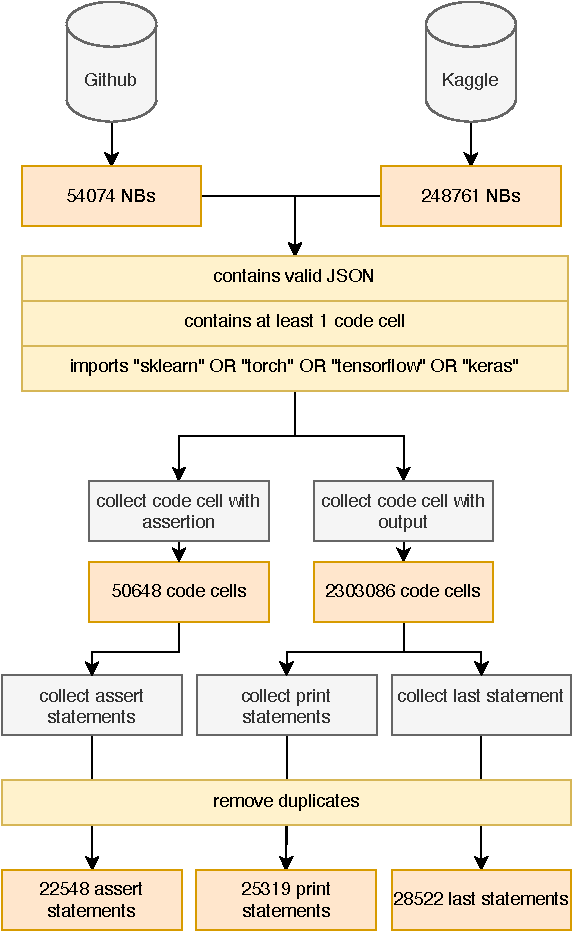
\includegraphics[width=\linewidth]{data-collection.pdf}
\label{fig:data-collection}
\caption{Overview of data collection methodology used in this study}
\end{figure}

Figure~\ref{fig:data-collection} summarises the data collection procedure used in this study. We collected Jupyter notebooks written in Python, from Kaggle and Github. 

We mined public repositories from Github to collect $49923$ Jupyter notebooks. We use the Github advanced search syntax~\footnote{https://docs.github.com/en/search-github/searching-on-github/searching-code} to isolate Jupyter Notebook that contain the keyword ``assert'' in them. The final search query is as follows: \texttt{"assert" language:"Jupyter Notebook"}.\footnote{Collected on June 22, 2023}

For Kaggle, we used a pre-existing dataset KGTorrent~\cite{quaranta2021kgtorrent} since Kaggle does not support advanced code-based search like Github. To the best of our knowledge, KGTorrent this is the largest dataset of Python Jupyter notebooks obtained from Kaggle consisting of $248763$ notebooks.

Therefore, we start with 283GB of data comprising of $298686$ Python Jupyter notebooks.

We check the validity of the underlying JSON structure in each notebook using the nbformat tool ~\footnote{https://nbformat.readthedocs.io/en/latest/}. Since the focus of this study is on the analysis of Python code, we only include notebooks that contain at least one code cell. Finally, to focus on Python code written specifically for ML projects, we only include notebooks that import popular ML libraries~\footnote{These libraries are derived from white literature---https://www.coursera.org/articles/python-machine-learning-library, https://www.geeksforgeeks.org/best-python-libraries-for-machine-learning, https://www.datacamp.com/blog/top-python-libraries-for-data-science, https://www.kdnuggets.com/2020/11/top-python-libraries-data-science-data-visualization-machine-learning.html, https://lp.jetbrains.com/python-developers-survey-2022}.

For explicit feedback using assertions, we programmatically analyse the JSON structure of the notebooks to isolate code cells. We collect Python assert statements from the code cells by constructing and subsequently parsing the Abstract Syntax Tree (AST) of the source code present in each cell.

\todo{TODO: justify why we didn't collect failures (strerr); that is more debugging? not the focus of this paper?}
Similarly, for implicit feedback, we first isolate code cells that produce an output. The output of a cell may either be from a ``print'' statement or the last statement of the cell. We collect both of them using the AST of the cell.

Finally, we remove duplicate data points (asserts, prints and last statements) resulting in a final data set of $22548$ assertions, $25319$ print statements and $28522$ last statements.

\subsection{Case Studies}

\todo{TODO: might need a visual aid here}

We allocated a fixed time resource of 100 hours to conduct the case study analysis of all candidates (assertions and cell outputs). To surface interesting candidates for the case studies, we apply NLP techniques as described below.

\todo{TODO: point out the poor quality of notebooks out there (we have citations for this); and the resulting noise in the assertions/outputs. Thats why we need to apply these tecniques to surface unique and interesting candidates!}

The assertions and cell outputs are first tokenised---special characters and alpha-numeric words shorter than two characters are removed. Two stop words namely ``assert'' and ``print'' are removed since they appear in all assertions and print statements respectively. The term frequency (TF) for all tokens is calculated and then normalised using their inter-document frequency (IDF) such that tokens thay appear less frequently are assigned a higher value.

We apply stratified random sampling to identify the candidates for the case study analysis. The sub-groups are created by adding TF-IDF of the tokens in each candidate to produce an aggregate value. The candidates are then divided into quartiles based on the aggregate value. A candidate is randomly drawn from each bin and analysed as an in-depth case study. The analysis is stopped when the time resource is exhausted.

During each case study, we analyse the code of the candidate to understand its purpose. Additionally, we analyse the entire code cell, the previous cell, next cell and the notebook's purpose to bring in rich context.

\section{Results}

\subsection{Implicit feedback from the output of code cells}

\subsubsection{Data distribution check ($N = 7$)}
% (O2, O4, O9, O14, O20, O25, O48)

\begin{table}
\centering
\caption{Examples of cell outputs used to verify distribution of data.}
\begin{tabular}{@{}m{0.05\textwidth} m{0.4\textwidth} m{0.3\textwidth}@{}}
\toprule
\emph{\textbf{Key}}&
\emph{\textbf{Code}}&
\emph{\textbf{Description}}\\
\midrule

O14&
\begin{lstlisting}
pd.pivot_table(train, index='Survived', values=['Age', 'SibSp', 'Parch', 'Fare'])
\end{lstlisting}&
Check the mean value of the specified features for each label in the target feature.\\

O48&
\begin{lstlisting}
x_train.describe()
\end{lstlisting}&
Check the descriptive statistics of the training data. The above statement is written immediately after normalising the features in the training data.\\

\bottomrule
\end{tabular}
\label{tab:distribution-check}
\end{table}

\begin{figure*}
\centering
\subcaptionbox{Check the distribution of the feature \texttt{Age} with-respect-to the labels in the target feature \texttt{Survived}.\label{fig:distribution-check-kdeplot}}{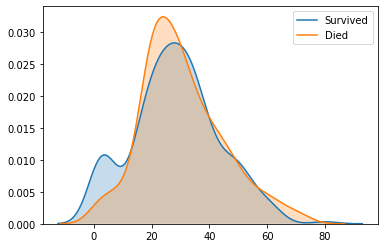
\includegraphics[width=0.45\linewidth]{distribution-check-kdeplot.png}}
\subcaptionbox{Check the distribution of the feature \texttt{likes} across all values of feature \texttt{category\_id}.\label{fig:distribution-check-catplot}}{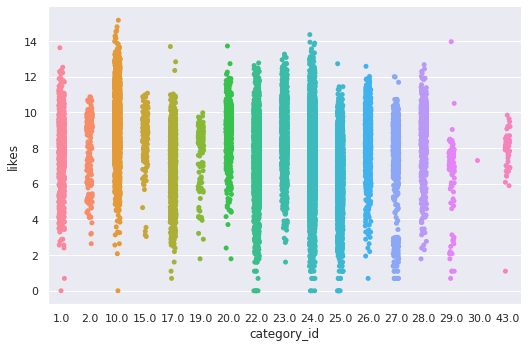
\includegraphics[width=0.45\linewidth]{distribution-check-catplot.png}}
\caption{Examples of visualisations used to check linear relationship in data.}
\label{fig:distribution-check}
\end{figure*}

Understanding the distribution of data is crucial for making informed decisions regarding necessary data transformation steps in data analysis processes. For instance, identifying whether scaling, normalizing, or handling outliers is required can be efficiently and effectively determined through visualizations.

% This is particularly important for models like linear regression, which perform optimally when data is normally distributed. If the data deviates from normality, additional transformation steps may be necessary to prepare it for training.


During the exploratory data analysis (EDA) or data understanding phase, a combination of visualizations and pandas dataframes is often employed to assess the distribution of specific columns within the data. This step helps identify features that may have a relationship with the target variable, ultimately informing which features to include in the machine learning model training process. This is seen in Figure~\ref{fig:distribution-check-kdeplot} where the distribution of a feature \texttt{Age} is checked against the labels of the target feature. Figure~\ref{fig:distribution-check-catplot} presents another example where the distribution of a continuous feature \texttt{likes} is checked with-respect-to all the values of another categorical feature \texttt{category\_id}.

For example, the distribution of a newly created feature, such as one where a continuous feature is binned into categories, is frequently examined. 

Descriptive statistics are also used post-transformation to verify that steps like data normalization have been effectively applied, ensuring that the data conforms to the expected format for further analysis.


Furthermore, distribution checks are often performed immediately after feature creation. For instance, this may occur after discretizing a continuous feature using binning. Additionally, descriptive statistics (e.g., mean and standard deviation) obtained from libraries like pandas can be used to verify the effectiveness of data normalization steps.

\subsubsection{Data relationship check ($N = 2$)}
% (O6, O10)
\todo{TODO: I think correlation checks should also be present in this group}

\begin{figure*}
\centering
\subcaptionbox{Using a lineplot to check linear relationship between two features in a dataset.\label{fig:linear-relation-check-lineplot}}{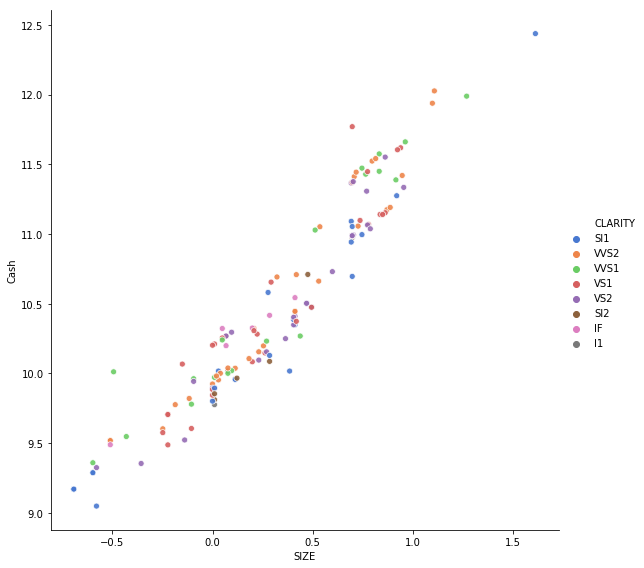
\includegraphics[width=0.45\linewidth]{linear-relation-check-lineplot.png}}
\subcaptionbox{Visualisation that shows the datapoints as a scatterplot along with a linear model fit.\label{fig:linear-relation-check-regplot}}{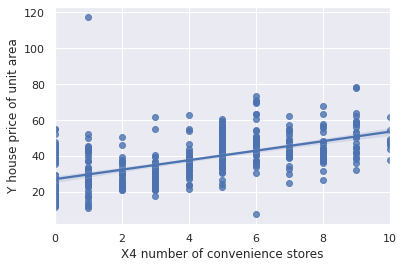
\includegraphics[width=0.45\linewidth]{linear-relation-check-regplot.png}}
\caption{Examples of visualisations used to check linear relationship in data.}
\label{fig:linear-relation-check}
\end{figure*}

Linear machine learning models achieve optimal performance when the target variable can be expressed as a linear combination of the input features. However, features within a dataset that exhibit a linear relationship are considered redundant as they convey the same information to the model during training. Consequently, the feature engineering stage often involves removing such features to create a more efficient training dataset~\ref{shome2022data}. Figure~\ref{fig:linear-relation-check} illustrates two methods for identifying these linear relationships. In Figure~\ref{fig:linear-relation-check-lineplot}, the practitioner assesses the linearity between the features \texttt{Cash} and \texttt{SIZE}. Figure~\ref{fig:linear-relation-check-regplot} depicts the visualization of the feature \texttt{X4} alongside the target variable \texttt{Y}, accompanied by a fitted linear regression model.

\subsubsection{Resource check ($N = 7$)}\label{sec:implicit-resource-check}
% (P71, P86, O64, O66, P68, P82, P107)

\begin{table}
\centering
\caption{Examples of cell outputs used to verify if different types of resources are available on the system where the notebook is being executed.}
\begin{tabular}{@{}m{0.1\textwidth} m{0.05\textwidth} m{0.4\textwidth} m{0.3\textwidth}@{}}
\toprule
\emph{\textbf{Type of resource}}&
\emph{\textbf{Key}}&
\emph{\textbf{Code}}&
\emph{\textbf{Description}}\\
\midrule

External library&
P71&
\begin{lstlisting}
print('Hub version: ', hub.__version__)
\end{lstlisting}&
Check the version of an external Python library installed on the current system.\\

Compute resources&
P68&
\begin{lstlisting}
print('GPU is available')
\end{lstlisting}&
Check if a GPU is available on the current system.\\

Data or pre-trained models&
O66&
\begin{lstlisting}
prostate_cancer_df.shape
\end{lstlisting}&
Check that the dataset has been loaded into memory.\\
\bottomrule
\end{tabular}
\label{tab:resource-check}
\end{table}

\todo{perhaps also add the keys of the case-studies here?}
Table~\ref{tab:resource-check} presents case studies where the output is used to verify that certain resources are available on the system in which the notebook is being executed. We find checks for the availability of compute resources (such as a GPU or a TPU), checking that the dataset or a pre-trained model has been loaded correctly and checks to ensure that a certain version of an external library is present on the system.

P71 highlights the lack of proper software engineering best practices within Jupyter notebooks. This shortcoming in computational notebooks has been identified by prior studies~\cite{quaranta2021kgtorrent, pimentel2019large-scale}. In this case study, managing dependencies through external tools is recommended. Python's built-in \emph{requirements.txt}~\footnote{https://pip.pypa.io/en/stable/reference/requirements-file-format/} file allows specifying dependencies and versions. Alternatively, external programs like \emph{pipenv}~\footnote{https://pipenv.pypa.io/en/latest/} and \emph{poetry}~\footnote{https://python-poetry.org/} use lockfiles to ensure specific version control, guaranteeing reproducibility across different systems. 

\subsubsection{Execution time check ($N = 1$)}
% (P66)

\begin{lstlisting}
print('Total Run Time:')
\end{lstlisting}

While training multiple machine learning models for a single task is common, choosing the best model considers not only its performance but also its training speed. Faster training times are more cost-effective for iterative tasks and promote sustainability in the long run. The provided code snippet (Listing~\ref{lst:exec-time-check}) exemplifies this concept by showcasing a case study (P66) that tracks training times for various models using a grid search. This approach allows practitioners to compare model performance alongside training efficiency. 

\subsubsection{Missing value check ($N = 3$)}
% (O12, O36, P74)

Checking for missing values is a critical step in the preprocessing phase of a machine learning project because it significantly influences the quality and performance of the model. Missing data can lead to biased or incorrect conclusions if not handled properly, potentially skewing the model's performance by training on incomplete or non-representative samples~\cite{shome2022data}. Many machine learning algorithms, including those that involve matrix multiplication operations such as linear regression and neural networks, demand complete numerical datasets to perform calculations. Missing values interrupt these calculations, leading to errors or the inability to execute algorithms entirely.

\begin{table}
\centering
\caption{Examples of cell outputs used to check for missing data.}
\begin{tabular}{@{}m{0.05\textwidth} m{0.6\textwidth}@{}}
\toprule
\emph{\textbf{Key}}&
\emph{\textbf{Code}}\\
\midrule

P74&
\begin{lstlisting}
print(train_df.isnull().sum())
\end{lstlisting}\\

O12&
\begin{lstlisting}
sns.heatmap(test_df.isnull(), yticklabels=False, cbar=False, cmap='viridis')
\end{lstlisting}\\

O36&
\begin{lstlisting}
test.isna().sum().unique()
\end{lstlisting}\\
\end{tabular}
\label{tab:missing-value}
\end{table}

Table~\ref{tab:missing-value} presents all case studies where cell outputs were used to check for missing data. While \emph{P74} and \emph{O36} perform this check in code, \emph{O12} presents a visual representation of missing data using a heatmap.

\subsubsection{Model performance check ($N = 33$)}
% (O3, O50, O52, O57, O74, P3, P6, P8--12, P16--19, P23, P24, P28, P30, P34, P42, P47, P48, P50, P51, P54, P55, P57, P58, P61, P78, P93)

\begin{table}
\centering
\caption{Various cell outputs used to check the performance of an ML model after training.}
\begin{tabular}{@{}m{0.05\textwidth} m{0.6\textwidth}@{}}
\toprule
\emph{\textbf{Key}}&
\emph{\textbf{Code}}\\
\midrule

P3&
\begin{lstlisting}
print('The mean accuracy with 10 fold cross validation is: %s ' % round(scores * 100, 2), '%')
\end{lstlisting}\\
    
P6&
\begin{lstlisting}
print('RMSE:', np.sqrt(metrics.mean_squared_error(y_test, pred)))
\end{lstlisting}\\

P18&
\begin{lstlisting}
print('The Accuracy is:', accuracy_score(y_test, y_pred))
\end{lstlisting}\\

P18&
\begin{lstlisting}
print('Classification Report: SVM (validation data)')
\end{lstlisting}\\

P54&
\begin{lstlisting}
print('Intercept value:', lm.intercept_)
\end{lstlisting}\\
\end{tabular}
\label{tab:model-perf}
\end{table}

The performance is printed to compare against other models/variations in the experimental model development phase; during the continuous experimentation phase, the author might change parameters of the model or change the data (engineer features, etc) and then re-run the model to check if the performance improved

Table~\ref{tab:model-perf} presents a few examples of cell outputs used to check the performance of a trained ML model. Besides \emph{accuracy}, we also see checks for the \emph{Root Mean Square Error (RMSE)} and the use of the classification report provided by scikit-learn~\footnote{https://scikit-learn.org/stable/modules/generated/sklearn.metrics.classification\_report.html}. In addition to the accuracy, the classification report also reports the \emph{precision}, \emph{recall} and \emph{f1 score} for all labels present in the target feature.

\emph{P54} prints the intercepts of a linear regression model. Checking the intercept of a linear regression model is essential for understanding the baseline prediction when all predictors are zero, interpreting the model, identifying potential data biases or missing variables, assessing model validity, and comparing baseline predictions across different models. This insight is critical for accurate model interpretation and effective decision-making in practical applications.

\begin{wrapfigure}{l}{0.45\linewidth}
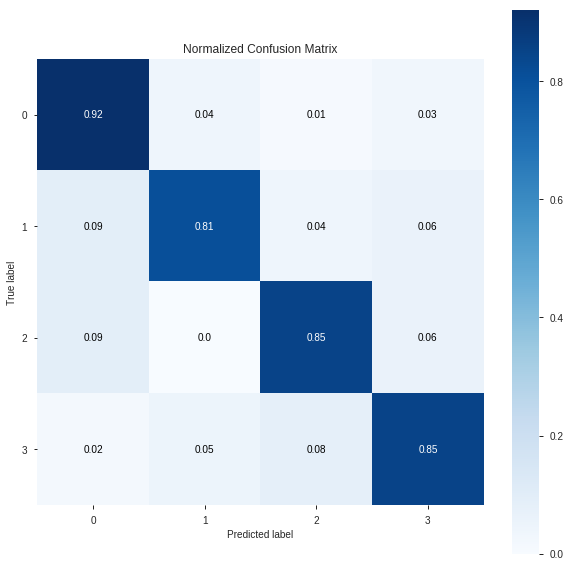
\includegraphics[width=\linewidth]{model-perf-confusion-matrix.png}
\caption{Confusion matrix}
\label{fig:model-perf-confusion-matrix}
\end{wrapfigure}

Figure~\ref{fig:model-perf-confusion-matrix} shows a heatmap used to visualise the confusion matrix of a multi-label classification task. The values are normalised using the actual number of examples of each class which makes the comparisons of the values across the classes possible.

% TODO: this looks horrible if we are wrapping text around the figure above
% \begin{lstlisting}[caption={Spot-check the performance of an image classification model for a random sample of input images.}, label={lst:model-perf-custom}]
% def spot_check_recs(classifier, seed):
%     random_images = []
%     random_labels = []
%     random_loc = np.random.randint(3000)
%     distance, loc = classifier.kneighbors( embedding_model.predict( visualize[random_loc].reshape(-1,28,28)), 100)
    
%     random_images.append(visualize[random_loc])
%     ...
%     for rec_loc, dist in zip(loc.reshape(-1,1), distance.reshape(-1,1)):
%         ...
        
%     ImageUtil.grid_display(random_images, random_labels, no_of_columns=1, figsize=(2,2), fig_title = "recs")

% spot_check_recs(classifier, 910)
% \end{lstlisting}

% Listing~\ref{model-perf-custom} shows a function implemented by a practitioners to manually evaluate an image classification model on a random sample of input images. The function prints the input image along with the prediction of the model which the practitioner uses to spot-check the performance of the model.

\subsubsection{Neural network architecture ($N = 1$)}
% (P92)

\begin{lstlisting}[caption={Print the architecture of a neural network.}, label={lst:network-architecture}]
print(MyNetwork)
\end{lstlisting}

Listing~\ref{lst:network-architecture} shows a print statement to show the architecture of a neural network. Printing the structure of a neural network serves crucial purposes such as verifying the correct implementation of the architecture, aiding in debugging by ensuring layer compatibility, and providing a clear, human-readable format for documentation and educational insights. It helps in verifying configurations like layer dimensions and operations before initiating computationally intensive training, ensuring the model is set up efficiently for the intended tasks. This practice is fundamental for maintaining accuracy, facilitating collaboration, and enhancing the reproducibility of the model.

\subsubsection{Shape check ($N = 3$}
% (P4, P32, P117)

Ensuring that data dimensions align with expectations is important particularly following data pre-processing or transformation steps.

Primarily, the number of features in the training set must match those in the testing set. This alignment is crucial because statistical machine learning models are trained on specific data dimensions and expect the same dimensional structure during inference to perform accurately. Similarly, in neural network architectures, the configuration of input layers depends directly on the shape of the training data, dictating the number of input neurons needed. Furthermore, the correspondence between the number of test examples and their respective labels is essential for accurately computing performance metrics, such as accuracy.

\begin{table}
\centering
\begin{tabular}{@{}m{0.05\textwidth} m{0.8\textwidth}@{}}
\toprule
\emph{\textbf{Key}} & \emph{\textbf{Code}}\\
\midrule
P4 &
\begin{lstlisting}
print('no.of examples in test data : ', len(test_data))
\end{lstlisting}\\
P32 &
\begin{lstlisting}
print('Training set shape : ', x_train.shape) 
\end{lstlisting}\\
\end{tabular}
\caption{Example of outputs used to check the shape of the data.}
\label{tab:shape-check}
\end{table}

Table~\ref{tab:shape-check} shows two print statements discovered in this study which demonstrate routine checks performed by developers to ensure the integrity and applicability of their models. Such checks are indicative of the meticulous attention to detail necessary in the model training and validation process, underscoring the importance of shape validation in achieving reliable machine learning outcomes.

\subsubsection{Type check ($N = 2$)}
% (O71, P43)

Ensuring data types align with model requirements is a fundamental step in the exploratory data analysis (EDA) phase of developing machine learning models. Since all machine learning algorithms perform mathematical operations, such as matrix multiplications, they require the input data to be entirely numerical to avoid computational errors. The process of checking data types helps in identifying the necessary pre-processing or transformation steps to convert the data into a form that is compatible with these models. For example, while numerical features often require normalisation to bring them within a specific scale, categorical features must be converted into a numerical format through methods like one-hot encoding to ensure they can be effectively integrated into the model.

This is illustrated in our analysis, where checks such as \texttt{print('data type:', images.dtype)} and \texttt{type(Y)} are employed to verify the data types of variables. These type checks are crucial not only for confirming the current state of the data but also for determining the specific transformations required to make the data suitable for subsequent modelling steps.

This proactive approach in the EDA phase facilitates smoother transitions into model training and can significantly impact the performance and effectiveness of the final machine learning models.

\subsubsection{Spot checks ($N = 5$)}
% (O56, O60, P64, P67, P114)

\begin{table}
\centering
\begin{tabular}{@{}m{0.05\textwidth} m{0.8\textwidth}@{}}
\toprule
\emph{\textbf{Key}}&
\emph{\textbf{Code}}\\
\midrule

O60 &
\begin{lstlisting}
X_pca.head()
\end{lstlisting}\\

P64 &
\begin{lstlisting}
print(np.max(cur[:, :, 1]))
\end{lstlisting}\\

P114 &
\begin{lstlisting}
print(onehot_encoded)
\end{lstlisting}\\
\end{tabular}
\caption{Example of outputs used to perform spot checks.}
\label{tab:spot-check}
\end{table}

Table~\ref{tab:spot-check} presents outputs which were used to spot check at various stages of the ML development cycle. Performing value or spot checks can be an essential practice for ensuring data integrity and model accuracy at various stages of development. These checks are crucial for verifying that operations such as data transformations, model predictions, and feature engineering are functioning as expected.

% The check in P67 involves a manual verification of the output of an activation function in a neural network, which is essential for confirming the functional efficacy of neural components in model training. 

In \emph{O60}, the analyst verifies that the number of features in the data matches expectations after apply Principal Component Analysis (PCA). This is a critical step for maintaining dimensional consistency in feature-reduced datasets. \emph{P64} demonstrates another case which is particularly relevant in image processing contexts. The maximum value in the second channel of a 3D numpy array is extracted and verified, ensuring that the data manipulation retains its expected properties. Lastly, \emph{P114} assesses the correctness of one-hot encoding, a fundamental preprocessing step for categorical data, ensuring that the transformation has been executed correctly.

Each of these checks not only validates individual transformations or predictions but also reinforces the overall reliability and robustness of the machine learning models being developed.

\subsubsection{Model training ($N = 4$)}
% (O8, O31, O42, P77)

\begin{table}
\centering
\begin{tabular}{@{}m{0.05\textwidth} m{0.8\textwidth}@{}}
\toprule
\emph{\textbf{Key}}&
\emph{\textbf{Code}}\\
\midrule

O8 &
\begin{lstlisting}
autoencoder.fit(x=X_train, y=X_train, epochs=15, validation_data=[X_test, X_test], callbacks=[keras_utils.TqdmProgressCallback()], verbose=0)
\end{lstlisting}\\

O31 &
\begin{lstlisting}
adaBoost.fit(X_train, y_train)
\end{lstlisting}\\

O42&
\begin{lstlisting}
m_r.best_params_
\end{lstlisting}\\
\end{tabular}
\caption{Example of outputs used to monitor model training.}
\label{tab:model-training}
\end{table}

The ``Model Training'' phase of ML workflows involves various critical activities, each aimed at ensuring effective model performance and robustness.

During training it is common practice to monitor progress periodically, as illustrated by outputs \emph{O8} in Table~\ref{tab:model-training}, where the training loss and accuracy are printed to give real-time feedback on the model's learning efficacy. This feedback allows for adjustments in training parameters or early stopping to prevent overfitting. For instance, in output O8, the autoencoder is trained using a custom callback from \texttt{keras\_utils} to provide a progress update without cluttering the output stream, which is particularly useful in lengthy training sessions. In contrast, output \emph{O31} represents a crucial validation step where the adaBoost model is fitted to the training data to ensure it adheres to the expected data patterns without errors, a typical task in the model experimentation phase where various models are assessed for their suitability. Output \emph{O42} possibly checks for the best parameters found through tuning methods, highlighting the importance of parameter optimisation in achieving optimal model performance.

Each of these outputs underscores different facets of the model training phase, from initialization and real-time monitoring to validation and finalization, illustrating the layered complexity of developing predictive models.

\subsection{Explicit feedback using \texttt{assert} statements}

% TODO: bring in the notion of pre and post condition checks (the wikipedia page on assertions is very interesting: https://en.wikipedia.org/wiki/Assertion_(software_development)); specifically the part on run-time assertions

\subsubsection{Batch size check ($N = 3$)}
% (A21, A28, A70)

\begin{table}
\centering
\begin{tabular}{@{}m{0.05\textwidth} m{0.8\textwidth}@{}}
\toprule
\emph{\textbf{Key}}&
\emph{\textbf{Code}}\\
\midrule

A21 &
\begin{lstlisting}
assert x.size(0) % batch_size == 0, f'the first dimension of input tensor ({x.size(0)}) should be divisible by batch_size ({batch_size})'
\end{lstlisting}\\

A28 &
\begin{lstlisting}
assert image_size % patch_size_small == 0, 'Image dimensions must be divisible by the patch size.'
\end{lstlisting}\\

A70 &
\begin{lstlisting}
assert n_img > batch_size
\end{lstlisting}\\
\end{tabular}
\caption{Assertions used to validate the batch size of input data.}
\label{tab:batch-size}
\end{table}

In the context of neural network training, the practice of using batch processing is a key strategy to enhance computational efficiency and hardware utilization, particularly GPU cores. Batching allows for a more stable and smoother learning curve as the model's weights are updated not for each individual example, but rather based on the average gradient of a batch. This technique not only optimizes learning but also enhances the model's generalizability due to more robust gradient estimations. Given these benefits, it becomes crucial to ensure that the batch size is appropriately set to match the hardware's capacity, avoiding memory overflow issues that can halt training.

Table~\ref{tab:batch-size} shows the assertions found in this study that validate the batch size. \emph{A21} ensure that the batch size divides evenly into the training dataset size, thereby confirming that every training epoch processes full batches without leftover data. Similarly, \emph{A28} checks that image dimensions are suitably divisible by the patch size, which is essential for certain types of convolutional networks. \emph{A70} is another critical check which confirms that the number of images is greater than the batch size, which is necessary to commence batch processing.

These assertions are strategically placed to prevent common errors that could undermine training efficiency and model performance, thereby safeguarding the training process from potential disruptions due to misconfigured batch sizes.

\subsubsection{Data leakage check ($N = 1$)}
% (A33)

Ensuring the absence of data leakage between training and validation datasets is a fundamental best practice in machine learning to prevent models from overfitting. Overfitting occurs when a model is excessively complex, learning not only the underlying patterns but also the noise in the training data, which can degrade its performance on unseen data. To guarantee that the model can generalize effectively to new examples, it's crucial to verify that the training and validation sets are completely distinct with no shared examples.

This is exemplified in assertion \emph{A33}, where the code \texttt{assert len(set( tr\_df.PetID.unique()).intersection(valid\_df.PetID.unique())) == 0} checks for this exact condition. This assertion ensures that there are no overlapping \texttt{PetID} values between the training set (\texttt{tr\_df}) and the validation set (\texttt{valid\_df}), thereby preventing any possibility of data leakage.

By strictly separating these datasets, the validation phase serves its purpose of providing an unbiased evaluation of the model's ability to generalize---to data similar to, but not identical to that which it was trained on---thus maintaining the integrity and validity of the evaluation metrics derived during model testing.

\subsubsection{Resource check ($N = 2$)}
% (A18, A67)

\todo{NOTE: connect this to~\ref{sec:implicit-resource-check}}

In the dynamic and sometimes unstructured environment of Jupyter notebooks, managing dependencies directly within the notebook becomes crucial due to the workflow peculiarities associated with interactive sessions. Unlike traditional software development environments where dependencies are managed through dedicated solutions like dependency management tools or by specifying requirements in a \emph{requirements.txt} file, notebooks often require on-the-fly checks to ensure the correct library versions are loaded to avoid compatibility issues.

This practice is illustrated by assertions such as those seen in \emph{A18} and \emph{A67}, where the code explicitly verifies the versions of critical libraries. For instance, \texttt{assert pd.\_\_version\_\_.rpartition(`.`)[0] == `1.0`} checks that the major version of pandas is precisely what is expected for the notebook’s tasks, ensuring compatibility and preventing errors that could arise from API changes in newer or older versions.

These assertions safeguard the notebook against potential disruptions caused by version mismatches, thereby maintaining the integrity of the codebase and ensuring reproducibility across different execution environments.

\subsubsection{Existence check ($N = 8$)}
% NOTE: this is a combination of missing-value-check and existence-check
% (A23, A42, A43, A50, A51, A63, A79, A86)

\begin{table}
\centering
\begin{tabular}{@{}m{0.05\textwidth} m{0.8\textwidth}@{}}
\toprule
\emph{\textbf{Key}}&
\emph{\textbf{Code}}\\
\midrule

A23 &
\begin{lstlisting}
assert np.all(orders.groupby('user_id') .days_since_prior_order.tail(1).notnull())
\end{lstlisting}\\

A42 &
\begin{lstlisting}
assert not lab_s.isnull().values.any()
\end{lstlisting}\\

A43 &
\begin{lstlisting}
assert len(data) != 0, 'cannot divide by zero'
\end{lstlisting}\\

A50 &
\begin{lstlisting}
assert not np.any(np.isnan(X))
\end{lstlisting}\\

A51 &
\begin{lstlisting}
assert data.target.notnull().all()
\end{lstlisting}\\

A63 &
\begin{lstlisting}
assert X.isnull().sum().sum() == 0
\end{lstlisting}\\

A79 &
\begin{lstlisting}
assert not processed_data_df.isna().any().any()
\end{lstlisting}\\

A86 &
\begin{lstlisting}
assert p0 in poi_info.index
\end{lstlisting}\\
\end{tabular}
\caption{Assertions used to perform existence checks.}
\label{tab:existence-check}
\end{table}

Existence checks are a fundamental component of data preprocessing in machine learning, serving multiple critical purposes to ensure data integrity before analysis and modeling. These checks primarily focus on verifying the presence of necessary columns and the absence of missing values within those columns. Such validations are especially crucial after data preprocessing steps, where transformations might inadvertently introduce null values.

For instance, assertions like \emph{A23} and \emph{A42} in Table~\ref{tab:existence-check} ensure that specific data columns do not contain any missing entries, which could compromise the reliability of subsequent analyses. Another common check, as seen with \emph{A43}, guards against operations on empty datasets, which are a potential risk after filtering or merging data processes. Similarly, checks such as \emph{A50}, \emph{A51} and \emph{A63} rigorously confirm that the datasets are entirely free from \texttt{NaN} values, thus preserving the integrity of the dataset for reliable model training. Additionally, assertions like \emph{A79} and \emph{A86} ensure that no unexpected missing values are introduced and that all expected indices are present in the dataset respectively.

These checks are crucial for maintaining the accuracy and efficiency of data handling processes, ensuring that the datasets are ready for robust machine learning applications.

\subsubsection{Mathematical property checks ($N = 4$)}
% (A3, A25, A56, A64)

\begin{table}
\centering
\begin{tabular}{@{}m{0.05\textwidth} m{0.8\textwidth}@{}}
\toprule
\emph{\textbf{Key}}&
\emph{\textbf{Code}}\\
\midrule

A3 &
\begin{lstlisting}
assert (xH - wH) % self.stride == 0
\end{lstlisting}\\

A25 &
\begin{lstlisting}
assert test_output.std() < 0.15, "Don't use batchnorm here"
\end{lstlisting}\\

A56 &
\begin{lstlisting}
assert np.allclose(e_v_states[:, -1], np.ones_like(e_v_states[:, -1]))
\end{lstlisting}\\

A64 &
\begin{lstlisting}
assert np.allclose(T, T.T)
\end{lstlisting}\\
\end{tabular}
\caption{Assertions used to validate mathematical properties of neural networks.}
\label{tab:maths-check}
\end{table}

When working with neural networks and other statistical models, it is imperative to ensure that mathematical properties are preserved throughout operations involving arrays and matrices. This rigor is captured through specific assertions aimed at validating these properties post-matrix manipulations.

Assertion \emph{A3} checks that the dimension differences between height of input and the filter, when divided by the stride, result in an integer, ensuring that convolution operations are dimensionally consistent. \emph{A25} monitors the standard deviation of outputs to decide the appropriateness of using batch normalisation, thus guiding the model optimization process based on statistical behavior. \emph{A56} verifies the uniformity of certain computations, essential for maintaining consistency in state or parameter arrays over iterations. Similarly \emph{A64} checks for the symmetry of a matrix, a crucial property in many algorithms, particularly those involving covariance matrices and distance calculations. 

These assertions are not just precautionary but are vital for confirming that the underpinnings of machine learning algorithms align with expected mathematical principles, thereby ensuring the robustness and reliability of model computations and outcomes.

\subsubsection{Model performance check ($N = 11$)}
% (A7, A15, A19, A22, A24, A26, A38, A54, A58, A59, A72)

\begin{table}
\centering
\begin{tabular}{@{}m{0.05\textwidth} m{0.8\textwidth}@{}}
\toprule
\emph{\textbf{Key}}&
\emph{\textbf{Code}}\\
\midrule

A7 &
\begin{lstlisting}
assert len(neighbours_1) == 20, "Neighbors don't match!"
\end{lstlisting}\\

A15 &
\begin{lstlisting}
assert np.allclose(verify('images/camera_1.jpg', 'bertrand', database, FRmodel), (0.54364836, True))
\end{lstlisting}\\

A19 &
\begin{lstlisting}
assert np.allclose(linear_model.coef_, [[1.57104472, 0.92521608]]), 'The model parameters you learned seem incorrect!'
\end{lstlisting}\\

A38 &
\begin{lstlisting}
assert 0.75 < auc(fpr, tpr) < 0.85
\end{lstlisting}\\

A58 &
\begin{lstlisting}
assert np.isclose(accuracy, 0.9666666666666667)
\end{lstlisting}\\
\end{tabular}
\caption{Assertions used to check performance of ML models.}
\label{tab:model-perf-explicit}
\end{table}

This study finds several assertions used to test model performance against predefined thresholds for key metrics such as accuracy, precision, recall, F1 score, and others.

For example, \emph{A7} in Table~\ref{tab:model-perf-explicit} checks for the expected number of neighbors, an indirect measure of model performance in specific scenarios like recommendation systems or clustering. Meanwhile, direct comparisons of model outputs with expected results, as seen in \emph{A15} validate the model's predictive accuracy and reliability under operational conditions. Other assertions, such as \emph{A19}, ensure that the learned parameters align closely with theoretically or empirically derived values, further cementing the model’s statistical validity. Additionally, range checks like \emph{A38} confirm that the performance metrics such as AUC and Gini coefficient fall within acceptable boundaries, indicating good predictive performance without overfitting. Additionally, the use of \texttt{np.isclose} in \emph{A58} is particularly noteworthy. This method accounts for the stochastic nature of many ML models, where slight variations in performance metrics can occur due to differences in initial conditions, random seed settings, or inherent randomness in algorithms. By allowing a small tolerance in the comparison, np.isclose ensures that the model's performance is consistently close to the expected benchmark, thereby affirming its reliability despite the stochastic elements.

Each assertion acts as a crucial checkpoint that verifies the model's ability to generalize and perform effectively, ensuring that the outcomes are both robust and trustworthy.

\subsubsection{Network architecture check ($N = 1$)}
% (A11)

When integrating pre-trained models or leveraging transfer learning techniques, it is crucial to ensure the compatibility of the custom neural network architecture with the pre-trained components. This is particularly important when combining convolutional layers from different sources, as the spatial dimensions and channel configurations must align correctly.

We encountered an \texttt{assert} statement that addresses this architectural compatibility check: \lstinline{assert self.encoder_conv_01[0].weight.size() == self.vgg16.features[2].weight.size()}. This assertion verifies that the weight dimensions of the first convolutional layer in the \lstinline{encoder_conv_01} module match the weight dimensions of the third layer in the \lstinline{vgg16.features} module. The \lstinline{vgg16} model is a widely-used pre-trained convolutional neural network often employed as a feature extractor or backbone for transfer learning tasks. By ensuring that the weight dimensions are consistent, the code guarantees that the input data to the \lstinline{encoder_conv_01} module has the expected spatial dimensions and number of channels, enabling seamless integration with the pre-trained \lstinline{vgg16} model.

This architectural check is crucial for preventing potential issues during the forward pass of the neural network and ensuring that the custom and pre-trained components are compatible, ultimately leading to reliable and accurate model performance.

\subsubsection{Resource check ($N = 5$)}
% (A10, A14, A37, A60, A74)

\begin{table}
\centering
\begin{tabular}{@{}m{0.05\textwidth} m{0.8\textwidth}@{}}
\toprule
\emph{\textbf{Key}}&
\emph{\textbf{Code}}\\
\midrule

A10 &
\begin{lstlisting}
assert le_path.is_file(), f"Label encoder file not found at {le_path}. Make sure 'label_encoder.pkl' exists in the lightning_logs directory."
\end{lstlisting}\\

A14 &
\begin{lstlisting}
assert self.model is not None, 'Model is not loaded, load it by calling .load_model()'
\end{lstlisting}\\

A37 &
\begin{lstlisting}
assert svm.fit_status_ == 0, 'Forgot to train the SVM!'
\end{lstlisting}\\

A60 &
\begin{lstlisting}
assert f2.gca().has_data()
\end{lstlisting}\\

A74 &
\begin{lstlisting}
assert os.path.exists(image_dir)
\end{lstlisting}\\
\end{tabular}
\caption{Assertions used to validate availability of resources.}
\label{tab:resource-check-explicit}
\end{table}

Ensuring the availability and integrity of required resources is a critical aspect of any machine learning workflow. Table~\ref{tab:resource-check-explicit} highlights some of the assertions we encountered that perform resource checks encompassing pre-trained models, data paths, visualizations, and model training status. These checks help prevent runtime errors and ensure the proper execution of code.

One set of assertions verify the existence of files on the file system, such as pre-trained models (\emph{A10}) or data files (\emph{A74}). These checks ensure that the required resources are present before proceeding with subsequent operations, preventing potential issues caused by missing files.

Additionally, assertions are employed to validate the successful loading of models (\emph{A14}) and the completion of model training processes (\emph{A37}). A unique aspect of working with notebooks is the ability to re-run cells while experimenting, which can lead to unintended consequences. The assertion \emph{A37} addresses this scenario by checking if the SVM model has been properly trained before proceeding with further operations. This check prevents inconsistent model states from executing cells out of order or multiple times.

Furthermore, assertions are used to verify the presence of data in visualizations generated using libraries like Matplotlib (\emph{A60}). These checks are crucial for ensuring that the visualizations accurately represent the underlying data and do not contain empty or incomplete plots, which could lead to misleading interpretations.

Resource check assertions play a vital role in maintaining the reliability and robustness of the machine learning workflows by ensuring the availability and validity of essential resources, preventing runtime errors, and maintaining the integrity of the data, models, and visualizations.

\subsubsection{Data shape check ($N = 26$)}
% (A5, A9, A13, A16, A17, A29, A31, A61, A71, A76--78, A82, A84, A85, A89, A90, A91, A93--96, A98--101)

Data shape checks can be considered the ``Swiss army knife''' of assertions, as they are ubiquitous and serve multiple purposes throughout the machine learning workflow. We encountered a vast array of assert statements that verify the dimensions of various data structures, including input features, labels, predictions, images, sequences, and embeddings. These assertions ensure that the data adheres to the expected format and dimensions required by different components of the machine learning pipeline.

For instance, assertions like \emph{A17}:~\lstinline{assert X.shape[1] == 13, 'Did you drop/lose some columns in X? Did you properly load and split the data?'} and \emph{A90}:~\lstinline{assert len(X_train) == 2000} verify that the input features have the correct number of columns and examples, respectively. Such checks are essential for preventing downstream errors and ensuring the compatibility of the data with the chosen model architecture and preprocessing steps.

Similarly, assertions like \emph{A5}:~\lstinline{assert y_valid.shape == (1132,)} and \emph{A29}~\lstinline{assert len(test_y_preds) == len(test_y), 'Unexpected number of predictions.'} ensure that the labels or predictions have the expected length or shape, which is crucial for accurate performance evaluation and model training.

In the context of computer vision tasks, assertions like \emph{A31}:~\lstinline{assert img.shape == (112, 92)} and \emph{A84}~\lstinline{assert red.get_shape().as_list()[1:] == [224, 224, 1]} verify that the input images have the correct dimensions, which is essential for compatibility with convolutional neural network architectures and image preprocessing techniques.

Furthermore, assertions like \emph{A76}:~\lstinline{assert len(encoding['token_type_ids']) == max_seq_length} and \emph{A93}:~\lstinline{assert temp_embed.shape[0] == stride} check the dimensions of sequences, embeddings, and other data structures used in natural language processing tasks, ensuring their compatibility with various models and algorithms.

Data shape check assertions serve as a crucial safeguard against data inconsistencies, ensuring the integrity and compatibility of the data throughout the machine learning workflow. By verifying the expected dimensions and shapes of various data structures, these assertions help prevent runtime errors, ensure accurate model training and evaluation, and maintain the reliability of the entire machine learning pipeline.

\subsubsection{Type check ($N = 5$)}
% (A2, A35, A40, A81, A88)

Type checking assertions play a crucial role in maintaining the integrity and consistency of data types throughout the machine learning workflow. In the examined notebooks, we encountered several assert statements that verify the types of input features, models, data structures, and other objects.

One common type check is performed on the input features, as demonstrated by the assertion \emph{A2}:~\lstinline{assert isinstance(X_trn, torch.FloatTensor), 'Features should be float32!'}. This assertion ensures that the input features are represented as PyTorch float tensors, which is a requirement for many deep learning models and operations.

Another type check is applied to verify the type of the machine learning models themselves. For instance, the \emph{A40}:~\lstinline{assert isinstance(model_3, sklearn.ensemble.RandomForestClassifier)} checks if the \lstinline{model_3} object is an instance of the \lstinline{RandomForestClassifier} class from the scikit-learn library. This type of assertion is essential when working with different types of models, as it helps prevent errors arising from using incompatible methods or attributes.

In addition to input features and models, type checks are also performed on data structures and intermediate objects. The assertion \emph{A35}:~\lstinline{assert isinstance(column_transformer, ColumnTransformer), "Input isn't a ColumnTransformer"} verifies that the \lstinline{column_transformer} object is an instance of the \lstinline{ColumnTransformer} class, which is commonly used for preprocessing and feature engineering tasks in scikit-learn.

Type checking is not limited to objects and data structures--it can also be applied to individual columns or elements within a dataset. The assertion \emph{A81}:~\lstinline{assert is_all_ints(filled_df[r]) is True} checks if all the elements in a specific column (\lstinline{filled_df[r]}) of a DataFrame are integers.

Furthermore, type checks are performed on NumPy arrays, as demonstrated by the assertion \emph{A88}:~\lstinline{assert isinstance(betas, np.ndarray)}. This assertion ensures that the \texttt{betas} object is a NumPy array, which is a fundamental data structure used in many numerical and scientific computing operations.

Type check assertions are essential for maintaining data integrity, ensuring compatibility between different components of the machine learning pipeline, and preventing errors and unexpected behavior. By verifying the types of input features, models, data structures, and other objects, these assertions contribute to the overall reliability and robustness of the machine learning workflow.

\subsubsection{Value check (A30, A41, A44--46, A52, A65, A68, A69, A73, A92)}

Check that the values in a column are in the specified values (categorical) or in a specified range (normalised continuous variable) or binary (such as the label column).

% NOTE: blanks and unit-tests
\subsubsection{Miscellaneous checks (A6, A20, A32, A34, A36, A53, A62, A75, A83, A87, A97)}

These feel like unit tests, performed in lieu of writing full test suites in the notebook.

%\begin{acknowledgements}
%If you'd like to thank anyone, place your comments here
%and remove the percent signs.
%\end{acknowledgements}


% Authors must disclose all relationships or interests that 
% could have direct or potential influence or impart bias on 
% the work: 
%
% \section*{Conflict of interest}
%
% The authors declare that they have no conflict of interest.


% BibTeX users please use one of
% \bibliographystyle{spbasic}      % basic style, author-year citations
\bibliographystyle{spmpsci}      % mathematics and physical sciences
%\bibliographystyle{spphys}       % APS-like style for physics
\bibliography{bibliography}   % name your BibTeX data base

\subsection{Assertions derived from visualisations}
\end{document}
% end of file template.tex

